\documentclass[12pt,a4paper]{article}
\usepackage[a4paper,margin=1in]{geometry}
\usepackage{graphicx}
\usepackage{booktabs}
\usepackage{amsmath,amssymb}
\usepackage{float}
\usepackage{hyperref}
\usepackage{xcolor}
\usepackage{listings}
\usepackage{enumitem}
\usepackage{fancyhdr}
\usepackage{longtable}
\hypersetup{colorlinks=true,linkcolor=blue,urlcolor=blue}
\pagestyle{fancy}
\fancyhf{}
\lhead{ICS1512}
\rhead{Machine Learning Algorithms Laboratory}
\cfoot{\thepage}
\lstset{
language=Python,
basicstyle=\ttfamily\small,
numbers=left,
frame=single,
breaklines=true,
showstringspaces=false
}
\begin{document}
\begin{tabular}{|p{4cm}|p{11cm}|}
\hline
Experiment No. & 5\\ \hline
Experiment Title & Decision Tree and Random Forest: A Comparative Classification Study\\ \hline
GitHub Repository & \url{https://github.com/Dharika-2006/ML-LAB-ASSIGMENTS} \\ \hline
Student Name & Dharika Shree K\\ \hline
Register Number & 3122247001014\\ \hline
Faculty & Dr. Poreddy Ajay Kumar Reddy \\ \hline
Submission Date & 02.08.26\\ \hline
\end{tabular}
\section{Objective}
To build and compare two ensemble-based classifiers Decision Tree and Random Forest — on the Wisconsin Diagnostic Breast Cancer dataset, tune their hyperparameters using 5-Fold Cross-Validation, and evaluate them using accuracy, precision, recall, F1-score, confusion matrices, ROC curves, AUC, and cross-validation performance.

\section{Problem Statement}
\textbf{Problem:}Classify breast cancer tumors as malignant or benign using Decision Tree and Random Forest classifiers, and compare their performance on the Wisconsin Diagnostic Breast Cancer dataset by tuning their hyperparameters using 5-Fold Cross-Validation and evaluating them using accuracy, precision, recall, F1-score, confusion matrices, ROC curves, and AUC.

\textbf{Input:} The Wisconsin Diagnostic Breast Cancer dataset, containing 569 samples with 30 numerical features describing characteristics of breast cell nuclei, with each sample classified as malignant or benign.

\textbf{Output:} Trained and tuned Decision Tree and Random Forest models, hyperparameter tuning results, confusion matrices, ROC curves, 5-fold cross-validation scores, and a final accuracy/precision/recall/F1-score comparison between the two algorithms.

\section{Dataset Description}
\begin{longtable}{|p{6cm}|p{8cm}|}
\hline
Dataset Name & Wisconsin Diagnostic Breast Cancer Dataset\\ \hline
Dataset Source & Scikit-learn\\ \hline
Number of Samples & 569\\ \hline
Number of Features & 30 \\ \hline
Number of Classes & 2 \\ \hline
Missing Values & None \\ \hline
Train-Test Split & 80\% training and 20\% testing\\ \hline
\end{longtable}

\section{Exploratory Data Analysis}
\begin{itemize}
\item Dataset overview
\item Statistical summary
\item Missing value analysis
\item Class distribution
\item Correlation matrix
\item Feature distribution
\end{itemize}

\subsection*{Figure: Class Distribution}
\begin{figure}[H]
\centering

\includegraphics[width=0.6\linewidth]{cld1.png}
\caption{Class distribution of benign and malignant samples}
\end{figure}
\textbf{Inference:}
The dataset contains 357 benign samples (approximately 62.7\%) and 212 malignant samples (approximately 37.3\%). Thus, the classes are not perfectly balanced, although the imbalance is not extreme. Since both classes have a substantial number of samples, the dataset is suitable for binary classification. The train-test split was stratified to preserve approximately the same class distribution in both the training and testing sets. Therefore, accuracy alone may not provide the complete picture, making precision, recall, and F1-score useful additional evaluation metrics.


\subsection*{Figure: Statistical Summary}

\includegraphics[width=0.5\linewidth]{summ.png}
\\
\textbf{Inference:}
The dataset contains 569 samples and 30 numerical features representing characteristics of breast cell nuclei. The target variable contains two classes, with 357 samples belonging to the benign class and 212 samples belonging to the malignant class. This corresponds to approximately 62.7\% benign and 37.3\% malignant samples, indicating a moderate class imbalance. The displayed feature values also show that the dataset contains measurements such as radius, texture, perimeter, area, smoothness, compactness, concavity, symmetry, and fractal dimension.

\subsection*{Figure: Correlation Matrix}
\begin{figure}[H]
\centering

\includegraphics[width=1\linewidth]{corr.png}
\caption{Feature correlation heatmap showing the relationships among the 30 numerical features in the dataset.}
\end{figure}
\textbf{Inference:}
The heatmap shows that several features are strongly positively correlated, particularly mean radius, mean perimeter, and mean area, as well as their corresponding worst measurements. Features such as compactness, concavity, and concave points also show noticeable positive correlations with one another. In contrast, some features such as texture error and fractal dimension-related features have weaker correlations with many other variables. Overall, the dataset contains several correlated features, indicating that some measurements provide similar information about the characteristics of the breast cell nuclei.

\section{Data Preprocessing}
\begin{itemize}
\item \textbf{Missing value handling:} No missing value handling was performed, as the dataset contains the required numerical feature values and no missing values were reported during the analysis.

\item \textbf{Encoding:} The target classes were mapped to numerical labels, with Malignant represented as 0 and Benign represented as 1. The 30 input features were already numerical and required no encoding.

\item \textbf{Feature scaling:} Not required. Decision Tree and Random Forest classifiers are tree-based models and do not require feature standardization or normalization.

\item \textbf{Train-test split:} The dataset was divided into 80\% training and 20\% testing sets using \texttt{train\_test\_split}, with \texttt{stratify=y} and \texttt{random\_state=42}. This produced 455 training samples and 114 testing samples while preserving the class distribution.

\item \textbf{Feature engineering:} None -- the original 30 numerical features were used directly for model training.
\end{itemize}

\section{Machine Learning Algorithm}

\subsection*{Decision Tree Classifier}

\textbf{Working principle:} A Decision Tree recursively splits the feature space into smaller regions using decision rules based on impurity measures. At each node, the algorithm selects a feature and split that best separates the classes. The splitting process continues until a stopping condition is reached.

\textbf{Mathematical formulation:}
For a node containing samples from different classes, the Gini impurity is given by
\[
G = 1-\sum_{k=1}^{K}p_k^2
\]
where $p_k$ is the proportion of samples belonging to class $k$. The split that produces the greatest reduction in impurity is selected.

Entropy can also be used as the splitting criterion:
\[
H = -\sum_{k=1}^{K}p_k\log_2(p_k)
\]

The main hyperparameters considered in this experiment are \texttt{criterion}, \texttt{max\_depth}, \texttt{min\_samples\_split}, and \texttt{min\_samples\_leaf}.

\textbf{Advantages:} Easy to interpret, capable of modelling non-linear decision boundaries, and does not require feature scaling. It can also capture feature interactions through hierarchical decision rules.

\textbf{Limitations:} A single Decision Tree can have high variance and is prone to overfitting, particularly when the tree becomes too deep. Tree depth and minimum sample parameters therefore need to be tuned carefully.

\subsection*{Random Forest Classifier}

\textbf{Working principle:} Random Forest is an ensemble learning method that combines multiple Decision Trees. Each tree is trained using a bootstrapped sample of the training data and a random subset of features. The final prediction is obtained through majority voting across the individual trees.

\textbf{Mathematical formulation:}
For a classification problem, the Random Forest prediction can be represented as
\[
\hat{y} = \operatorname{mode}
\left\{
T_1(x),T_2(x),\ldots,T_B(x)
\right\}
\]
where $T_b(x)$ represents the prediction of the $b$-th decision tree and $B$ is the total number of trees.

The main hyperparameters explored in this experiment are \texttt{n\_estimators}, \texttt{max\_depth}, \texttt{max\_features}, and \texttt{bootstrap}.

\textbf{Advantages:} Reduces the variance associated with a single Decision Tree, improves stability and generalization through ensemble learning, and does not require feature scaling.

\textbf{Limitations:} More computationally expensive than a single Decision Tree because multiple trees must be trained. It also has more hyperparameters to tune, and the resulting model is less interpretable than an individual Decision Tree.
\section{Experimental Setup}
\begin{tabular}{ll}
\toprule
Python Version & Python 3 (Google Colab runtime)\\
Scikit-Learn Version & As installed in the Google Colab environment\\
IDE & Google Colaboratory (Jupyter-based notebook)\\
Operating System & Linux (Google Colab backend)\\
Hardware & Google Colab-provided CPU runtime\\
\bottomrule
\end{tabular}

\section{Hyperparameter Selection}
\begin{tabular}{ll}
\toprule
Parameter & Value\\
\midrule
Train-Test Split & 80:20, stratified, \texttt{random\_state=42}\\
Cross-Validation & 5-fold, scoring = accuracy\\
Decision Tree -- search space & \texttt{criterion} $\in\{\texttt{gini},\texttt{entropy}\}$,\\
& \texttt{max\_depth} $\in\{3,5,7,10,\texttt{None}\}$,\\
& \texttt{min\_samples\_split} $\in\{2,5,10\}$,\\
& \texttt{min\_samples\_leaf} $\in\{1,2,4\}$\\
Decision Tree -- best params & \texttt{criterion=gini}, \texttt{max\_depth=5},\\
& \texttt{min\_samples\_split=5}, \texttt{min\_samples\_leaf=1}\\
Decision Tree -- best CV Accuracy & 0.9385\\
Random Forest -- search space & \texttt{n\_estimators} $\in\{50,100,200\}$,\\
& \texttt{max\_depth} $\in\{5,10,\texttt{None}\}$,\\
& \texttt{max\_features} $\in\{\texttt{sqrt},\texttt{log2}\}$,\\
& \texttt{bootstrap} $\in\{\texttt{True},\texttt{False}\}$\\
Random Forest -- best params & \texttt{n\_estimators=100}, \texttt{max\_depth=None},\\
& \texttt{max\_features=log2}, \texttt{bootstrap=False}\\
Random Forest -- best CV Accuracy & 0.9692\\
\bottomrule
\end{tabular}

\section{Results}
\begin{longtable}{lcccc}
\toprule
Model & Accuracy & Precision & Recall & F1-score\\
\midrule
Decision Tree (tuned) & 0.9211 & 0.9565 & 0.9167 & 0.9362\\
Random Forest (tuned) & 0.9561 & 0.9589 & 0.9722 & 0.9655\\
\bottomrule
\end{longtable}

\noindent The tuned Random Forest clearly outperforms the Decision Tree, achieving 95.61\% accuracy compared to 92.11\%. It also achieves higher recall (97.22\% vs.\ 91.67\%) and F1-score (96.55\% vs.\ 93.62\%), while maintaining a slightly higher precision (95.89\% vs.\ 95.65\%). The Random Forest also obtained a best 5-fold cross-validation accuracy of 96.92\%, indicating strong generalization performance. Overall, the ensemble approach provides better classification performance and stability than the single Decision Tree on this dataset.

\section{Result Visualization}
Include all graphs generated during the experiment.

\subsection*{1. Correlation Matrix}
See Section 4 -- several features show strong positive correlations, particularly mean radius, mean perimeter, and mean area, along with their corresponding worst measurements. Features related to compactness, concavity, and concave points also show noticeable correlations, indicating that some variables capture related characteristics of the breast cell nuclei.

\subsection*{2. Class Distribution}
See Section 4 -- the dataset contains 357 benign samples (62.7\%) and 212 malignant samples (37.3\%). The classes are therefore moderately imbalanced, making stratified train-test splitting and metrics such as precision, recall, and F1-score useful for evaluation.
\subsection*{3. Confusion Matrix}

\begin{figure}[H]
\centering

\includegraphics[width=0.55\linewidth]{conf1.png}
\caption{Confusion Matrix -- Decision Tree}
\end{figure}

\begin{figure}[H]
\centering

\includegraphics[width=0.55\linewidth]{conf2.png}
\caption{Confusion Matrix -- Random Forest}
\end{figure}

\textbf{Inference:}
The Decision Tree produced 9 misclassifications, with 3 false positives and 6 false negatives. In comparison, the Random Forest produced only 5 misclassifications, with 3 false positives and 2 false negatives. Thus, the Random Forest reduces both the overall number of errors and the number of false negatives, which is reflected in its higher recall and F1-score. Overall, the Random Forest provides better classification performance than the Decision Tree on the test set.
\subsection*{4. ROC Curve}

\begin{figure}[H]
\centering
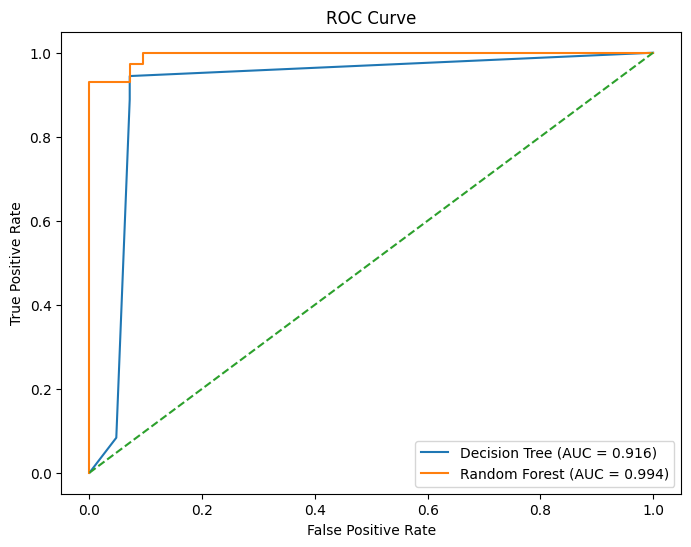
\includegraphics[width=0.75\linewidth]{roc.png}
\caption{ROC Curve -- Decision Tree and Random Forest}
\end{figure}

\textbf{Inference:}
The ROC curves illustrate the trade-off between the true positive rate and false positive rate for the two classifiers. The Random Forest is expected to show stronger overall discrimination than the Decision Tree, consistent with its higher test accuracy, recall, and F1-score. The AUC values provide an additional measure of how effectively the models distinguish between the two classes.

\subsection*{5. Precision-Recall Curve}
Not generated separately in the notebook; the evaluation focused on accuracy, precision, recall, F1-score, confusion matrices, and ROC curves. However, the reported precision and recall values provide a useful comparison: the Random Forest achieves higher recall (0.9722) and a slightly higher precision (0.9589) than the Decision Tree (0.9167 recall and 0.9565 precision). This indicates that the Random Forest is better at identifying the positive class while maintaining a similar level of precision.

\subsection*{6. Model Comparison}

\begin{figure}[H]
\centering

\includegraphics[width=0.7\linewidth]{comp.png}
\caption{Accuracy comparison between the tuned Decision Tree and Random Forest}
\end{figure}

\textbf{Inference:}
The Random Forest outperforms the tuned Decision Tree, achieving 95.61\% test accuracy compared to 92.11\% for the Decision Tree. The ensemble model also achieves higher recall and F1-score, while maintaining a slightly higher precision. This improvement demonstrates the benefit of combining multiple decision trees through ensemble learning, which reduces variance and provides better generalization than a single Decision Tree.

\subsection*{7. Learning Curve}
Hyperparameter tuning was performed using 5-fold cross-validation with GridSearchCV to select the best-performing Decision Tree and Random Forest configurations.

\subsection*{8. Feature Importance}

\begin{figure}[H]
\centering
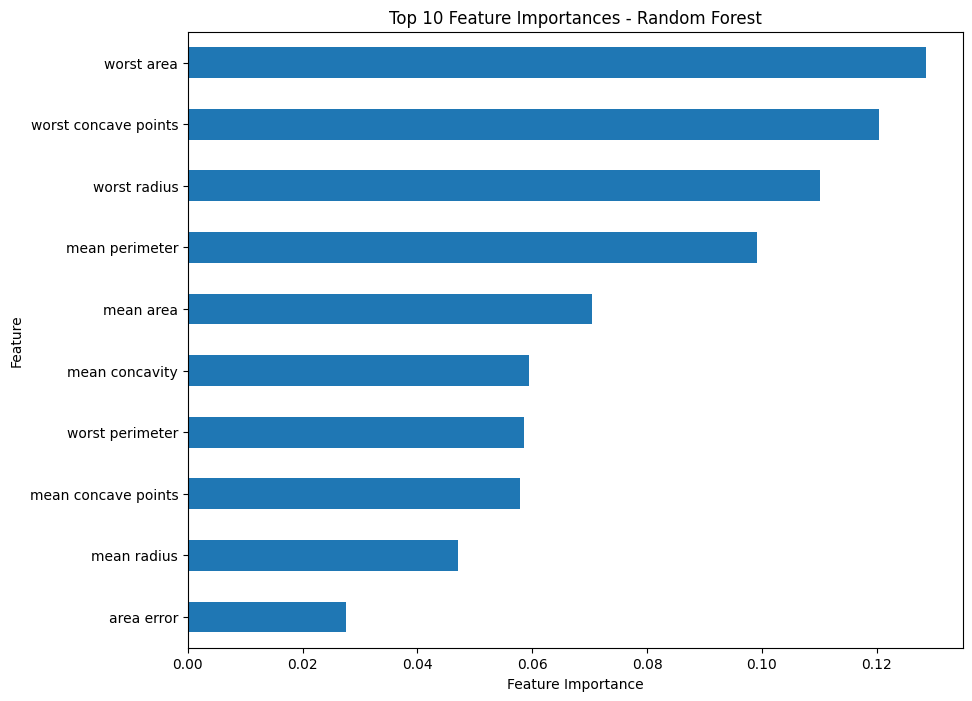
\includegraphics[width=0.7\linewidth]{feat.png}
\caption{Top 10 Feature Importances -- Random Forest}
\end{figure}

\textbf{Inference:}
The Random Forest feature-importance analysis shows that \textit{worst area} is the most influential feature, followed by \textit{worst concave points} and \textit{worst radius}. Other highly important features include \textit{mean perimeter}, \textit{mean area}, \textit{mean concavity}, and \textit{worst perimeter}. This indicates that measurements related to the size, shape, and irregularity of the breast cell nuclei contribute strongly to the model's classification decisions. Overall, the feature-importance results provide an indication of which characteristics are most useful for distinguishing between benign and malignant tumors.

\section{Discussion}

The Decision Tree and Random Forest both performed well on the Wisconsin Diagnostic Breast Cancer dataset, with accuracies of 92.11\% and 95.61\%, respectively. The Random Forest achieved higher recall and F1-score while maintaining a similar precision to the Decision Tree. Its 5-fold cross-validation accuracy of 96.92\% also indicates strong generalization performance. The confusion matrix showed that Random Forest made fewer misclassifications, particularly reducing false negatives. Feature importance identified worst area, worst concave points, and worst radius as the most influential features. Overall, the results demonstrate that the Random Forest provides better and more stable classification performance than a single Decision Tree.

\section{Conclusion}

This experiment compared Decision Tree and Random Forest classifiers for binary classification on the Wisconsin Diagnostic Breast Cancer dataset. After hyperparameter tuning using 5-fold cross-validation, the Random Forest achieved higher test accuracy, recall, and F1-score than the Decision Tree. The Random Forest obtained 95.61\% accuracy compared to 92.11\% for the Decision Tree, along with a cross-validation accuracy of 96.92\%. It also produced fewer misclassifications, demonstrating improved stability and generalization. Feature-importance analysis showed that worst area, worst concave points, and worst radius were among the most influential features. Overall, the results demonstrate that the Random Forest ensemble provides better classification performance than a single Decision Tree for this dataset.

\section{References}
\begin{enumerate}
\item Scikit-learn developers, Decision Trees, scikit-learn documentation: \url{https://scikit-learn.org/stable/modules/tree.html}

\item Scikit-learn developers, Random Forests, scikit-learn documentation: \url{https://scikit-learn.org/stable/modules/ensemble.html#random-forests}

\item UCI Machine Learning Repository, Wisconsin Diagnostic Breast Cancer Dataset: \url{https://archive.ics.uci.edu/}
\end{enumerate}
\end{document}